%\documentclass[a4paper,twoside]{ctexart}
\documentclass[a4paper,twoside]{article}
\usepackage[UTF8]{ctex}
\usepackage{geometry}
\geometry{margin=1cm,vmargin={0pt,1cm}}
\setlength{\topmargin}{-2cm}
\setlength{\paperheight}{23cm}
\setlength{\paperwidth}{18cm}
\setlength{\textheight}{19.6cm}
\setlength{\textwidth}{15cm}
\usepackage{makecell}
%\usepackage{fancyhdr}
\usepackage{siunitx}
\usepackage{amssymb}
\usepackage{indentfirst}
\setlength{\parindent}{0.5em}

\pagenumbering{arabic} 

% useful packages.
\usepackage{multirow}
\usepackage{caption}
\usepackage{mathrsfs}
\usepackage{amsfonts}
\usepackage{amsmath}
\usepackage{amsthm}
\usepackage{enumerate}
\usepackage{xcolor,graphicx,float,subfigure}
\usepackage{epstopdf}
\usepackage{multicol}
\usepackage{fancyhdr}
\usepackage{layout}
\usepackage{listings}
\lstset{language=Matlab}
\lstset{breaklines}
\lstset{extendedchars=false}
\usepackage[colorlinks,linkcolor=blue]{hyperref}
\usepackage{xcolor}
%\usepackage{cite}
%\usepackage[numbers,sort&compress]{natbib} 
%\setcitestyle{open={},close={}}
%\usepackage{natbibspacing}
%\renewcommand{\refname}{}
\usepackage{anyfontsize}

\newtheorem{theorem}{定理}[section]
\newtheorem{corollary}[theorem]{推论}
\newtheorem{lemma}[theorem]{引理}
\newtheorem{definition}[theorem]{定义}
\newtheorem{proposition}[theorem]{性质}
\newtheorem{example}[theorem]{例子}
\newtheorem{notation}[theorem]{记号}
\newtheorem{algorithm}[theorem]{算法}

%\pagestyle{plain}
\pagestyle{fancy}
\fancyhf{}
\fancyhead[LE,RO]{\textbf{\thepage}}

\makeatletter
\newcommand\sixteen{\@setfontsize\sixteen{17pt}{6}}
\renewcommand{\maketitle}{\bgroup\setlength{\parindent}{0pt}
\begin{flushleft}
\sixteen\bfseries \@title
\medskip
\end{flushleft}
\textit{\@author}
\egroup}
\makeatother

%\CTEXsetup[format={\Large\bfseries}]{section}

\title{三维殷集中的三角形求交问题数学文档}


\begin{document}
\maketitle
\section{本课题要解决的问题:}
实现高效的三角形求交算法。三维殷集的边界是由三角网格近似的,无论是对两个殷集求交还是对一个殷集求补,都会涉及到一个基本的问题:给定一堆三角形,如何求出它们所有的交线?之前我们的做法是对任两个三角形判断一次是否相交,这样做的时间复杂度是$O(N^2)$,其中$N$为三角形个数。这样的做法无疑是很浪费的,因为能够相交的三角形在空间上必定是挨着的,相距很远的三角形是不可能相交的,这也是二维扫描线算法的思想。我们希望利用这个事实减少需要判断相交的三角形对的个数,从而实现高效的三角形求交算法。






\section{拟采取的技术路线:}
本节的方法和图片参考\cite{octgpu}。

\subsection{均匀空间划分}
我们希望用空间划分法(spatial subdivision)加速三角形求交:将需要三角形求交的殷集(可能是一个也可能是多个)中的三角形放到一个容器中,用一个大的长方体包含所有三角形,对这个大长方体进行若干次划分,每次划分将已有长方体的$x,y,z$方向上的长度都减小一半,那么最终得到的空间划分是一系列长方体,它们包含了所有的三角形,如果一个三角形同时与多个长方体相交,默认每个长方体中都含有这个三角形,从而对每一个三角形,它只可能与它所在的长方体当中的三角形相交。利用这种空间划分,减少了需要判断相交的三角形对的个数,从而提高了求交效率。事实上,上述划分过程就是建立一棵八叉树的过程,初始的大长方体对应根节点,在三维空间中每次划分都将大长方体平分成8个小长方体,这对应父结点的八个子结点。当三角形的分布均匀时,这种均匀划分空间方法的时间复杂度是$O(N\text{log}(N))$。然而,当三角形的分布非常不均匀时,会出现许多长方体不包含三角形,而有些长方体包含很多三角形,这样求交的时间复杂度就会趋向$O(N^2)$。解决方案是设计一种自适应的办法,使得包含三角形多的长方体多划分几次,包含三角形少的少划分几次(见图\ref{fig:1})。

 \begin{figure}[H]
    \centering
    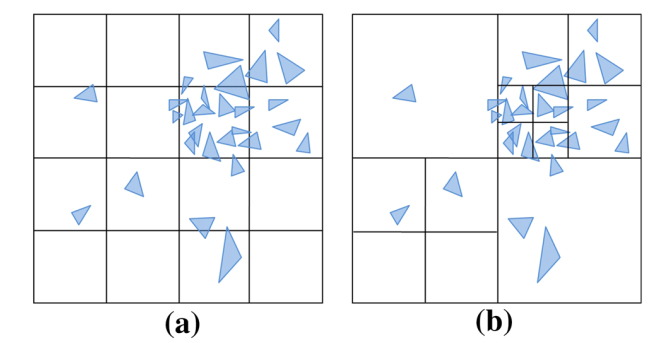
\includegraphics[width=1\linewidth]{png/1.png}
    \caption{对一个不均匀的三角形分布,(a)给出了均匀的空间划分,(b)给出了不均匀的空间划分。}
    \label{fig:1}
  \end{figure}
  

\subsection{单阶段自适应空间划分}
  为了实现自适应的效果,需要制定一个规则来决定一个长方体是否需要划分。由于我们的目标是尽可能减少三角形求交的次数,并且一个长方体内的$n$个三角形求交所需的次数$n(n-1)/2$是已知的,一个自然的想法是:如果对一个长方体进行划分后,每个小长方体内所需的三角形求交次数之和小于大长方体中三角形求交次数,那么就进行这次划分(见图\ref{fig:2}),否则就不划分(见图\ref{fig:3}),递归地对划分后的长方体也进行判断。上述的空间划分都是从上到下的,即把大长方体不断划分成小长方体,事实上,这个过程的逆过程(从下到上)同样也是可行的,也即从一个最细的划分开始,不断将小长方体合并成大长方体,那么上述的规则就可以修改为:如果合并后大长方体内所需的三角形求交次数小于合并前小长方体中三角形求交次数之和,就进行合并,反之则不合并。



\begin{figure}[H]
    \centering
    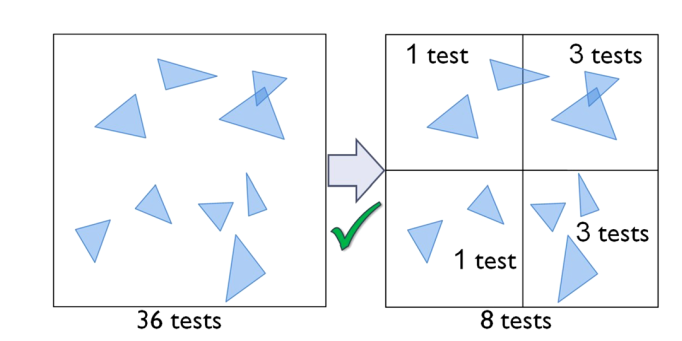
\includegraphics[width=0.8\linewidth]{png/2.png}
    \caption{划分减小了求交次数,接受。}
    \label{fig:2}
\end{figure}

\begin{figure}[H]
    \centering
    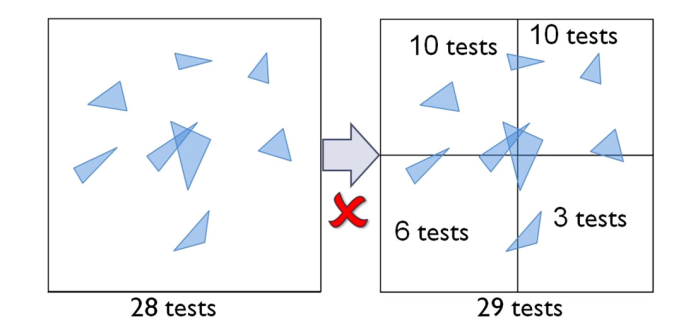
\includegraphics[width=0.8\linewidth]{png/3.png}
    \caption{划分增加了求交次数,拒绝。}
    \label{fig:3}
\end{figure}

与均匀划分相比,上述两种单阶段的自适应方法无疑减少了三角形求交的次数。然而这两种方法在一些情况下仍然是低效的:对于从上到下的自适应划分,可能会出现第一次划分增加了求交次数然而后续的几次划分极大地减少了求交次数的情况(见图\ref{fig:4});类似的,对于从下到上的自适应合并,可能会出现第一次合并增加了求交次数然而后续的几次合并极大地减少了求交次数的情况(见图\ref{fig:5})。为了处理这一类情况,一种解决办法是记录下每种可能出现的划分或合并情况所需的三角形求交次数,这样做的代价很大,因为情况数是以指数增加的。下面给出一种经济有效的自适应划分方法。

\begin{figure}[H]
    \centering
    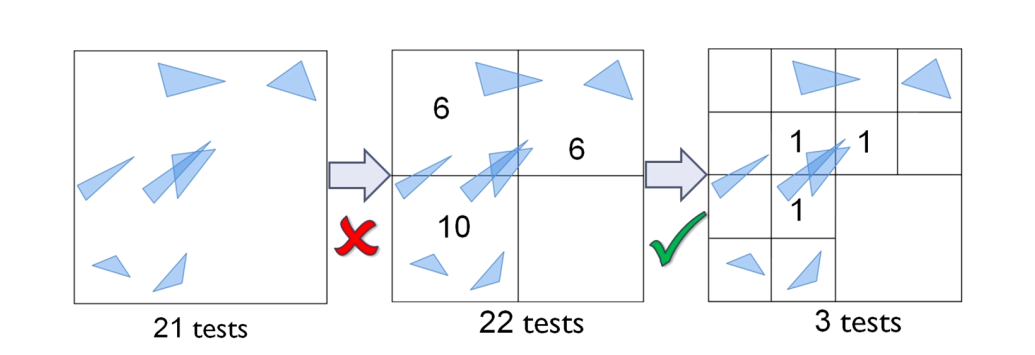
\includegraphics[width=1\linewidth]{png/4.png}
    \caption{从上到下的自适应划分的局限性。}
    \label{fig:4}
\end{figure}

\begin{figure}[H]
    \centering
    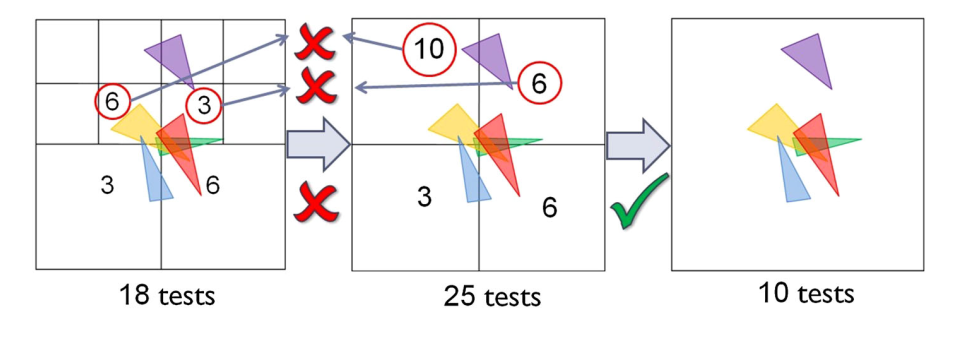
\includegraphics[width=1\linewidth]{png/5.png}
    \caption{从下到上的自适应合并的局限性。}
    \label{fig:5}
\end{figure}

\subsection{两阶段自适应空间划分}
我们采用两阶段的自适应方法。

\textbf{输入:}需要求交的三角形集。

\textbf{输出:}一棵实现了空间自适应划分的八叉树,其叶结点包含了需要两两求交的三角形。

\textbf{步骤:}预设置一个最细的划分,从最大的长方体逐步划分到最小的长方体,这个过程构成了一棵完全八叉树,我们用数组来表示这棵八叉树,数组长度等于八叉树的结点数。遍历每个三角形,让每个包含这个三角形的长方体都记录下三角形的序号,最小的长方体存储三角形的信息。遍历操作结束后,每个长方体包含的三角形数已知,所以每个长方体所需的三角形求交数也已知,将其存储到八叉树数组中。然后进行第一阶段:从下到上的合并。按照从下到上的遍历顺序,对每个父结点,若其八个子结点的值的和小于等于父结点的值,则将父结点的值改为八个子结点的值的和;若八个子结点的值的和大于父结点的值,则将父结点标记为叶结点。重复上述操作直到到达根结点。在经过上述阶段后,分支当中最高的叶结点是八叉树真正的叶结点(也即最终合并成的长方体),所以第二阶段只需从上到下遍历,找到这些叶结点。具体实现时,只需从根结点开始往下遍历,遇到叶结点时将其储存的值和其所有子树中的叶结点储存的值替换为它的序号,遍历结束后所有储存值和序号相同的叶结点就是八叉树真正的叶结点。从而,我们实现了自适应的空间划分。图\ref{fig:6}给出了一个一维情况下的例子。


\begin{figure}[H]
    \centering
    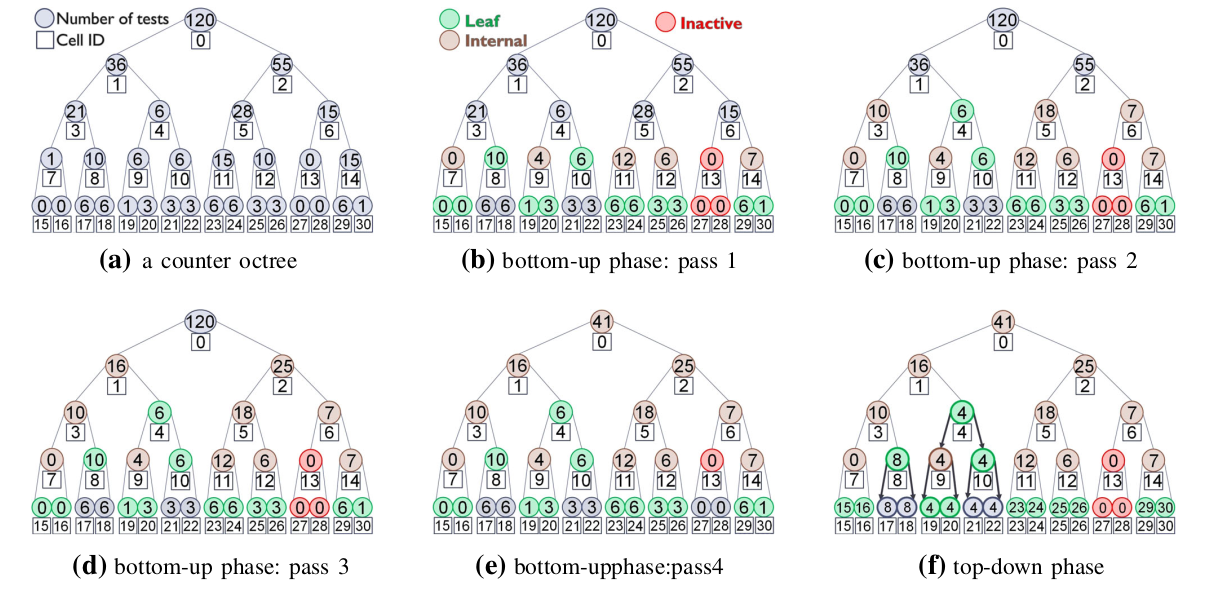
\includegraphics[width=1\linewidth]{png/6.png}
    \caption{两阶段自适应方法。}
    \label{fig:6}
\end{figure}


对于两阶段自适应方法得到的八叉树,我们将其每个叶结点中的三角形两两求交,就得到了所有的交线。


\section{当前的进展:}
已经看完了相关论文,开始写设计文档和程序。


\section{遇到的困难:}
上述的方法是可以用gpu加速的,但我们对于gpu的工作方式不是很熟悉,还需要去学习。


\bibliographystyle{unsrt}
\bibliography{bib/YinSets3D}
\end{document}
 